% This text will be sanitized and placed into lqa-output/abstract.txt
%
Motivation and approach: the trie index works for scaling sublinerly with the
reference size but each error in the query triggers deeper exploration of the
trie so the runtime grows exponentially. Lets inform the \A algorithm using
information from the whole query length while keeping the trie. This way we
could avoid the deep trie exploration and scale to long queries (as far as the
error rate is not too high).

We present a novel \A \emph{\seedh} that enables fast and optimal
sequence-to-graph alignment, guaranteed to minimize the edit distance of the
alignment assuming non-negative edit costs.

We phrase optimal alignment as a shortest path problem and solve it by
instantiating the \A~algorithm with our \seedh. The \seedh first extracts
non-overlapping substrings (\emph{seeds}) from the read, finds exact seed
\emph{matches} in the reference, marks preceding reference positions by
\emph{crumbs}, and uses the crumbs to direct the \A search. The key idea is to
punish paths for the absence of foreseeable seed matches. We prove admissibility
of the \seedh, thus guaranteeing alignment optimality.

\qquad Our implementation extends the free and open source aligner and
demonstrates that the \seedh outperforms all state-of-the-art optimal aligners
including \graphaligner, \vargas, \pasgal, and the \prefixh previously employed
by \astarix. Specifically, we achieve a consistent speedup of >60$\times$ on
both short Illumina reads and long HiFi reads (up to 25kbp), on both the
\textit{E.~coli} linear reference genome (1Mbp) and the MHC variant graph
(5Mbp). Our speedup is enabled by the \seedh consistently skipping >99.99\% of
the table cells that optimal aligners based on dynamic programming
compute.\\

\astarix aligner and evaluations: \astarixurl\\

Genome graph, Optimal alignment, Semi-global alignment, Edit distance, Shortest
path, Long reads, \A algorithm, Seed heuristic
\section{Overview}

\paragraph{Contributions}
%
Here we address the key challenge of scaling to long HiFi reads, while
retaining the superior scaling of \astarix in the size of the reference graph.
%
To this end, we instantiate the \A algorithm with a novel \seedh, which
outperforms existing optimal aligners on both short and long HiFi reads.
%
Specifically, the \seedh utilizes information from the whole read to narrowly
direct the \A search by placing \emph{crumbs} on graph nodes which lead up to a
\emph{seed match}, \ie, an exact match of a substring of the read.

Overall, the contributions presented in this chapter include:
\begin{enumerate}
    \item A novel \A~\seedh that exploits information from the whole read to
    quickly align it to a general graphs reference.
    \item An optimality proof showing that the \seedh always finds an alignment
    with minimal edit distance.
	\item An implementation of the \seedh as part of the \astarix aligner.
    \item An extensive evaluation of our approach, showing that we align both
    short Illumina reads and long HiFi reads to both linear and graph references
    $\geq 60 \times$ faster than existing optimal aligners.
    \item A demonstration of superior empirical runtime scaling in the reference
    size $N$: $N^{0.46}$ on Illumina reads and $N^{0.11}$ on HiFi reads.
\end{enumerate}

\begin{figure}[t]
    \centering
	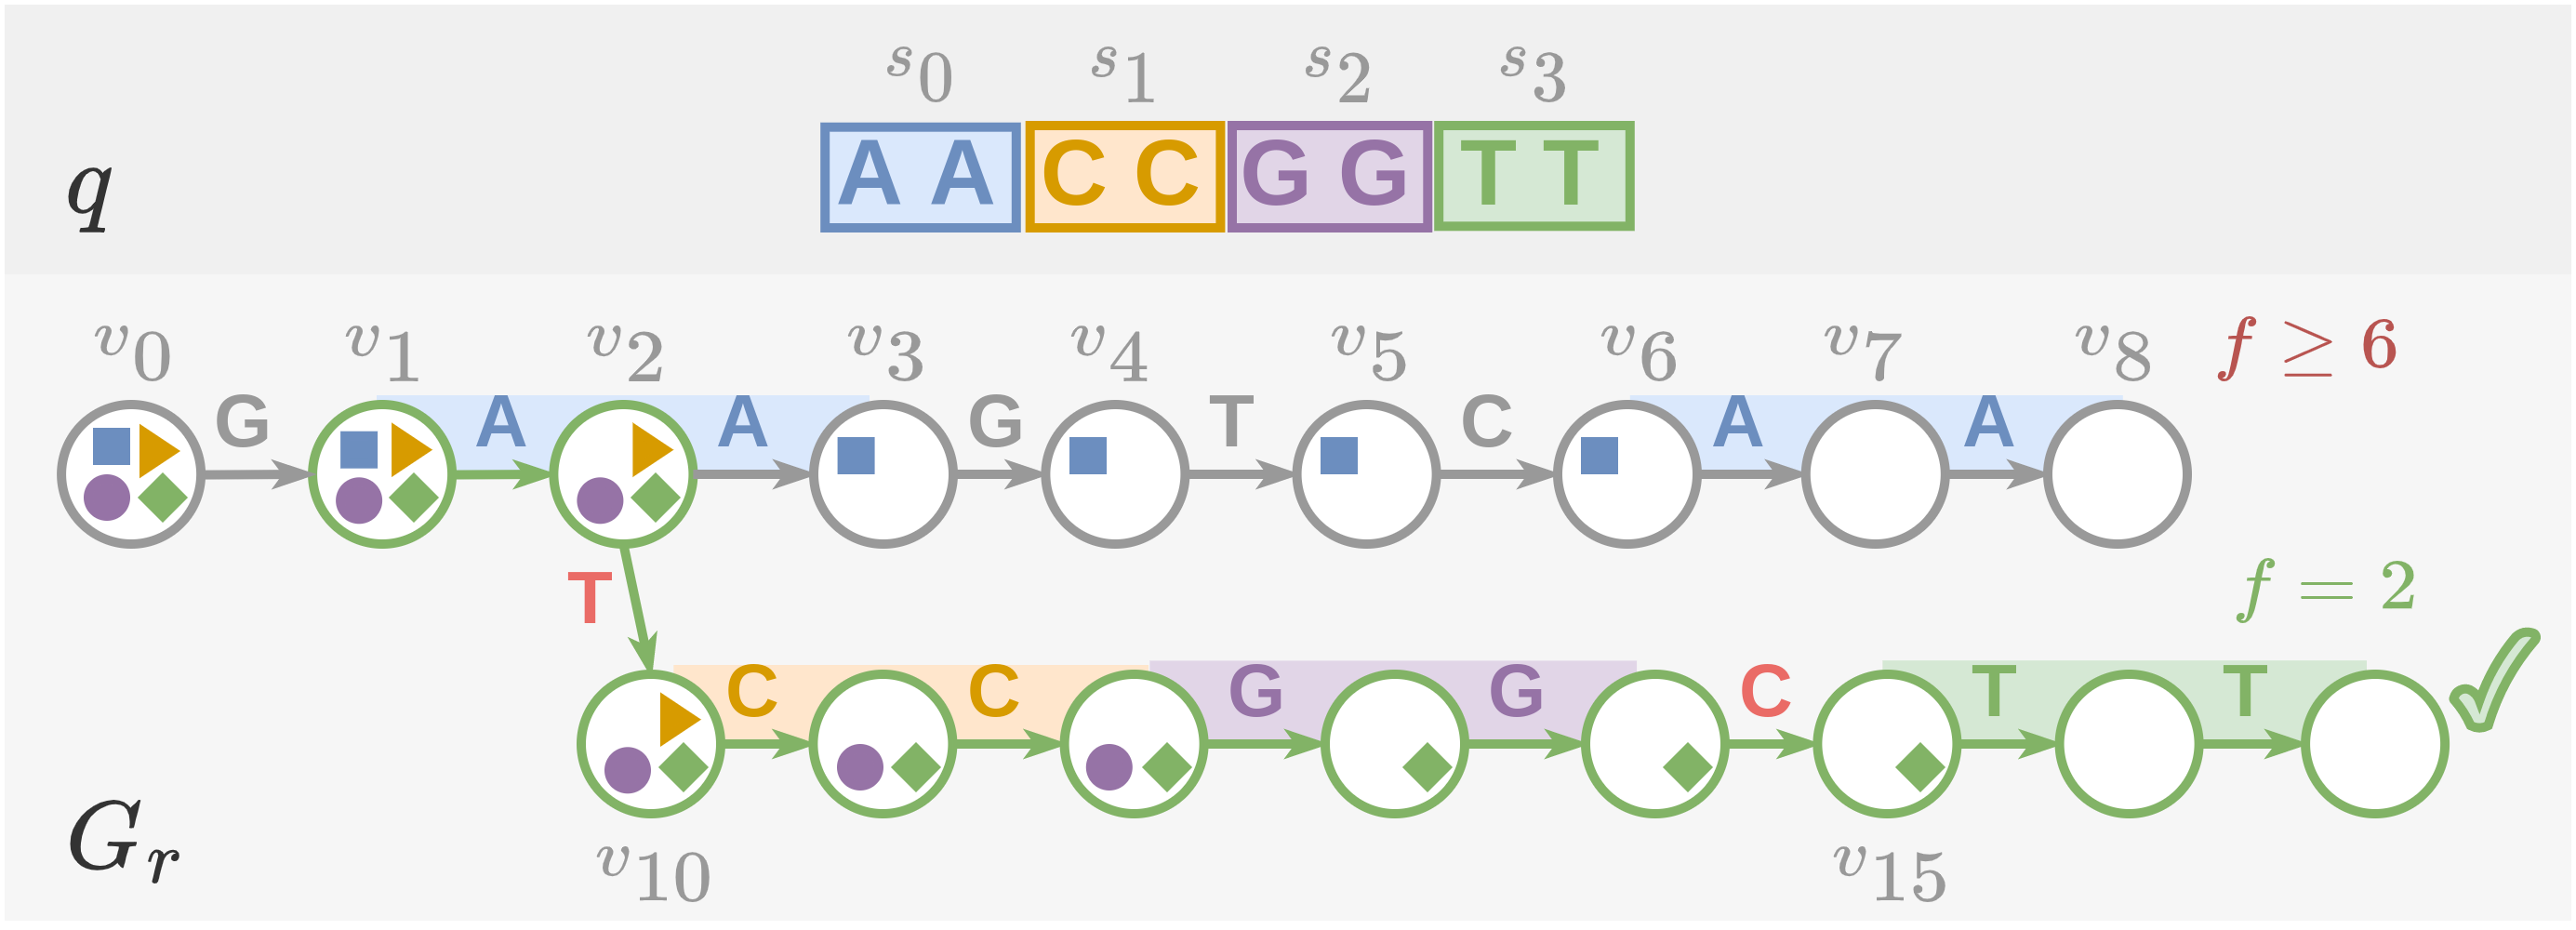
\includegraphics[width=0.6\linewidth]{figures/seed-heuristic-diagram.png}
	\caption{%
		A toy overview example using the \seedh to align a read $q$ to a
		reference graph $\RG$. The read is split into four colored seeds, where
		their corresponding crumbs are shown inside reference graph nodes as
		symbols with matching color. The optimal alignment is highlighted as a
		green path ending with a tick (\protect\greentick{}) and includes one
		substitution
		($\mathtt{\textcolor{dark-red}{T}{\rightarrow}\textcolor{dark-red}{A}}$)
		and one deletion ($\textcolor{dark-red}{\mathtt{C}}$).
		%
	}
\label{SEEDfig:overview}
\end{figure}

\paragraph{Intuition} \label{SEEDsec:overview}
% Task
\cref{SEEDfig:overview} showcases the \sh on an overview example. It shows a
read~$q$ to be aligned to a reference graph~$\RG$. Our goal is to find an
optimal alignment starting from an arbitrary node $v \in \RG$.
%
For simplicity of the exposition, we assume unit edit costs $\cedits =
(0,1,1,1)$, which we generalize in~\cref{SEEDsec:definition}.

\paragraph{Intuition}
The \A search requires us to provide a lower bound of the remaining path cost
from a state $\st{v}{i}$ to a target state. Clearly, to align the whole query,
each of the remaining seeds (\ie~at or after position $i$ in $q$) has to be
eventually aligned. The intuition underlying the \sh is to punish the state
for the absence of any foreseeable match of each remaining seed. Notice that the
order of the seeds is not directly taken into account.

In order to quickly check if a seed $s$ can lead to a match, we follow a
procedure similar to the one used by Hansel and Gretel who were placing
breadcrumbs to find their trail back home. Before aligning a query, we will
precompute all $\emph{crumbs}$ from all seeds so that not finding a crumb for
a seed $s$ on node $v$ indicates that seed $s$ could not be matched exactly
before the query is fully aligned continuing from $v$. This way, assuming that a
shortest path includes many seed matches, the crumbs will direct the \A search
along with it.

If a crumb from an expected seed is missing in node $v$, its corresponding seed
$s$ could not possibly be aligned exactly and this will incur the cost of at
least one substitution, insertion, or deletion. Assuming unit edit costs,
$h\st{v}{i}$ yields a lower bound on the cost for aligning $q[i{:}]$ starting
from $v$ by simply returning the number of missing expected crumbs in $v$.

\paragraph{Crumbs precomputation example}
%
\cref{SEEDfig:overview} shows four seeds as colored sections of length $2$ each, and
represents their corresponding crumbs as \bluecrumb{}, \yellowcrumb{},
\violetcrumb{} and \greencrumb{}, respectively. Four crumbs are expected if we
start at $v_2$, but \bluecrumb{} is missing, so $h\st{v_2}{0}=1$. Analogously,
if we reach $v_2$ after aligning one letter from the read, we expect 3 crumbs
(except \bluecrumb{}), and we find them all in $v_2$, so $h\st{v_2}{1}=0$.
%
To precompute the crumbs for each seed, we first find all positions in $\RG$
from which the seed aligns exactly. \cref{SEEDfig:overview} shows these exact
matches as colored sections of $\RG$. Then, from each match we traverse $\RG$
backwards and add crumbs to nodes that could lead to these matches.
%
For example, because seed \colorbox{light-yellow}{$\mathtt{CC}$} can be matched
starting in node $v_{10}$, crumbs~\yellowcrumb{} are placed on all nodes leading
up to $v_{10}$.
%
Similarly, seed \colorbox{light-blue}{$\mathtt{AA}$} has two exact matches, one
starting in node $v_{0}$ and one starting in node $v_{6}$.
%
However, we only add crumbs \bluecrumb{} to nodes $v_{0}$, $v_{1}$, and
$v_{3}$--$v_{6}$, but not to node $v_{2}$. This is because $v_{2}$ is
(i)~strictly after the beginning of the match of
\colorbox{light-blue}{$\mathtt{AA}$} at $v_1$ and (ii)~too far before the match
of \colorbox{light-blue}{$\mathtt{AA}$} at $v_{6}$.
%
Specifically, any alignment starting from node $v_{2}$ and still matching
\colorbox{light-blue}{$\mathtt{AA}$} at $v_{6}$ would induce an overall cost of
$4$ (it would require deleting the $4$ letters $A$, $G$, $T$, and $C$). Even
without a crumb \bluecrumb{} on $v_{2}$, our heuristic provides a lower bound on
the cost of such an alignment: it never estimates a cost of more than~$4$, the
number of seeds.

% In contrast to \bluecrumb{}, the crumbs \greencrumb{} for the match of seed
% \colorbox{light-green}{$\mathtt{TT}$} are placed on all nodes before $v_{15}$.
% This is because even when starting from $v_0$, we could match
% \colorbox{light-green}{$\mathtt{TT}$} at $v_{15}$ without a cost exceeding the
% cost of $4$ (by deleting $\mathtt{G}$, substituting
% $\mathtt{\textcolor{dark-red}{T}{\rightarrow}\textcolor{dark-red}{A}}$, and
% deleting $\mathtt{\textcolor{dark-red}{C}}$, at an overall cost of $3$).

\stepcounter{footnote}
\footnotetext{\label{SEEDfootnote:tie-braking}Depending on how the \A~algorithm
handles tie-braking, different sets of states could be explored. For simplicity,
we show all states that \emph{could potentially} be explored.}
\begin{figure}[t]
    \centering
	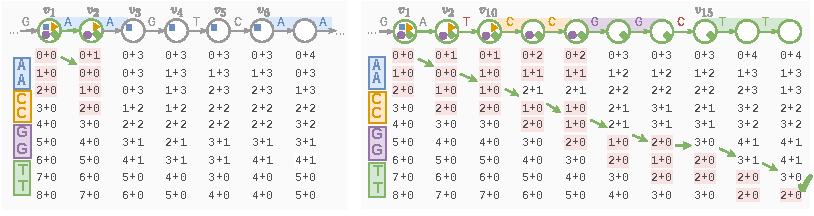
\includegraphics[width=\linewidth]{\dir/figures/seed-heuristic-tables}
	\caption{Exploration of $\AG[q]$, searching for a shortest path from the
	first to the last row using the \seedh. The table entry in the $i^\text{th}$
	row (zero indexed) below node $v$ shows $g\st{v}{i}+h\st{v}{i}$, where
	$g\st{v}{i}$ is the shortest distance from any starting state $\st{u}{0}$ to
	$\st{v}{i}$.
	%
	States that may\textsuperscript{\cref{SEEDfootnote:tie-braking}} be expanded by
	the \A~algorithm are highlighted in \colorbox{pink-highlight}{pink}, and the
	rest of the states are shown for completeness even though they are never
	expanded. The shortest path corresponding to the best alignment is shown
	with green arrows~(\textcolor{dark-green}{$\pmb{\rightarrow}$}).}
	%
	\label{SEEDfig:exploration-table}
\end{figure}


\paragraph{Guiding the search example}
%
\cref{SEEDfig:exploration-table} demonstrates how $h\st{v}{i}$ guides the
\A~algorithm towards the shortest path by showing which states may be
\colorbox{pink-highlight}{expanded} when using the \sh.
%
Specifically, the unique optimal alignment in \cref{SEEDfig:overview} starts from
node $v_{1}$, continues to $v_{2}$, and then proceeds through node $v_{10}$
(instead of~$v_{3}$).

While the \sh initially explores all states of the form $\st{v}{0}$ (we
discuss in \cref{SEEDsec:trie} how to avoid this by using a trie), it skips
expanding any state that involves nodes $v_{3}$--$v_{8}$. This improvement is
possible because all these explored states are penalized by the \sh by at
least $3$, while the shortest path of cost $2$ will be found before considering
states on nodes $v_{3}$--$v_{8}$.
%
Here, the heuristic function accurately predicts that expanding $v_{10}$ may
eventually lead to an exact alignment of seeds
\colorbox{light-yellow}{$\mathtt{CC}$}, \colorbox{light-violet}{$\mathtt{GG}$}
and \colorbox{light-green}{$\mathtt{TT}$}, while expanding $v_3$ may not lead to
an alignment of either seed.
%
In particular, the \sh is not misled by the short-term benefit of correctly
matching $A$ in $v_{2}$, and instead provides a long-term recommendation based
on the whole read. Thus, even though the walk to $v_{3}$ aligns exactly the
first two letters of $q$, \A does not expand $v_{3}$ because the \sh
guarantees that the future cost will be at least $3$.

% Overall, the \sh directs the search to the best alignment with one
% substitution
% ($\mathtt{\textcolor{dark-red}{T}{\rightarrow}\textcolor{dark-red}{A}}$) and
% one deletion ($\textcolor{dark-red}{\mathtt{C}}$).
